%%%%%%%%%%%%%%%%%%%%%%%%%%%%%%%%%%%%%%%%%%%%%%%%%%%%%%%%%%%%%%%%%%%%%%%%%%%%%%%%%%%%%%%%%%%%%%%%%%%%%%%
%%													%%
%% 	BAKALÁŘSKÁ PRÁCE -  Zásuvný modul QGIS pro pozemní monitorování radiace			%%
%% 				 Michael Kala							%%
%%													%%
%% pro formátování využita šablona: http://geo3.fsv.cvut.cz/kurzy/mod/resource/view.php?id=775 	%%
%%													%%
%%%%%%%%%%%%%%%%%%%%%%%%%%%%%%%%%%%%%%%%%%%%%%%%%%%%%%%%%%%%%%%%%%%%%%%%%%%%%%%%%%%%%%%%%%%%%%%%%%%%%%% 

\documentclass[%
  12pt,         			% Velikost základního písma je 12 bodů
  a4paper,      			% Formát papíru je A4
  oneside,       			% Oboustranný tisk
  pdftex,				    % překlad bude proveden programem 'pdftex' do PDF
%%%  draft
]{report}       			% Dokument třídy 'zpráva'
%

\newcommand{\Fbox}[1]{\fbox{\strut#1}}

\usepackage[czech, english]{babel}	% použití češtiny, angličtiny
\usepackage[utf8]{inputenc}		% Kódování zdrojových souborů je UTF8

\usepackage[square,sort,comma,numbers]{natbib}

\usepackage{caption}
\usepackage{subcaption}
\captionsetup{font=small}
\usepackage{enumitem} 
\setlist{leftmargin=*} % bez odsazení

\makeatletter
\setlength{\@fptop}{0pt}
\setlength{\@fpbot}{0pt plus 1fil}
\makeatletter

\usepackage[dvips]{graphicx}   
\usepackage{color}
\usepackage{transparent}
\usepackage{wrapfig}
\usepackage{float} 
\usepackage{listings}


\usepackage{cmap}           
\usepackage[T1]{fontenc}    

\usepackage{textcomp}
\usepackage[compact]{titlesec}
\usepackage{amsmath}
\addtolength{\jot}{1em} 

\usepackage{chngcntr}
\counterwithout{footnote}{chapter}

\usepackage{acronym}

\usepackage[
    unicode,                
    breaklinks=true,        
    hypertexnames=false,
    colorlinks=true, % true for print version
    citecolor=black,
    filecolor=black,
    linkcolor=black,
    urlcolor=black
]{hyperref}         

\usepackage{url}
\usepackage{fancyhdr}
%\usepackage{algorithmic}
\usepackage{algorithm}
\usepackage{algcompatible}
\renewcommand{\ALG@name}{Pseudokód}% Update algorithm name
\def\ALG@name{Pseudokód}

\usepackage[
  cvutstyle,          
  bachelor           
]{thesiscvut}


\newif\ifweb
\ifx\ifHtml\undefined % Mimo HTML.
    \webfalse
\else % V HTML.
    \webtrue
\fi 

\renewcommand{\figurename}{Obrázek}
\def\figurename{Obrázek}

%%%%%%%%%%%%%%%%%%%%%%%%%%%%%%%%%%%%%%%%%%%%%%%%%%%%%%%%%%%%%%%%%
%%%%%%%%%%% Definice informací o dokumentu  %%%%%%%%%%%%%%%%%%%%%
%%%%%%%%%%%%%%%%%%%%%%%%%%%%%%%%%%%%%%%%%%%%%%%%%%%%%%%%%%%%%%%%%

%% Název práce
\nazev{ Zásuvný modul QGIS pro pozemní~monitorování~radiace}
{QGIS Plugin for Ground Radiation Monitoring     }

%% Jméno a příjmení autora
\autor{Michael}{Kala}

%% Jméno a příjmení vedoucího práce včetně titulů
\garant{Ing.~Martin~Landa,~Ph.D.}

%% Označení oboru studia
\oborstudia{Geodézie, kartografie a~geoinformatika}{}

%% Označení ústavu
\ustav{Katedra geomatiky}{}

%% Rok obhajoby
\rok{2017}

%Mesic obhajoby
\mesic{červen}

%% Místo obhajoby
\misto{Praha}

%% Abstrakt
\abstrakt {Cílem této bakalářské práce je implementace softwarového
  nástroje umožňujícího plánování optimálních tras pozemního
  monitorování radiace. Při únicích radioaktivních látek do ovzduší je
  specializovanými softwary spočtena prognóza šíření radioaktivního
  mraku. Jedním z~produktů této prognózy je také mapa dávkových
  příkonů záření gama pro zasaženou oblast. Na základě této mapy
  vytvářený softwarový nástroj určí přibližný odhad dávky záření,
  kterou obdrží mobilní skupina provádějící měření na dané trase
  v~postiženém území. V~případě překročení hraničních hodnot nástroj
  pomůže v~přeplánování trasy přes jiné komunikace příp. změny
  doporučené rychlosti jízdy vozidla tak, aby mobilní skupina nebyla
  vystavována nebezpečným dávkám.}  {The~aim of this bachelor thesis
  is the~implementation of a~software tool enabling the~management of
  routes of the~ground radiation monitoring. During nuclear disasters,
  the~radioactive substances pollute the environment. Specialized
  softwares are capable of making a~prediction of the~spread of
  the~radiation cloud. One of the~products of the~prediction is also
  a~map of dose rates of the~gamma radiation. Based on this map,
  the~created software tool calculates an estimate of the~gamma
  radiation dose which a~mobile group doing the~field work would
  obtain on a~given route. In case the~dose limit value is exceeded,
  the~tool helps to plan changes of the~route waypoints using other
  roads or to modify the~recommended speed of the~vehicle so the~field
  mobile group would not obtain those values of the~dose, that are
  dangerous or even lethal.}

%% Klíčová slova
\klicovaslova
{GIS, QGIS, zásuvný~modul, python, SÚRO, ionizující záření, radiační ochrana}
{GIS, QGIS, plugin, python, NRPI, ionizing radiation, radiological protection}

%%%%%%%%%%%%%%%%%%%%%%%%%%%%%%%%%%%%%%%%%%%%%%%%%%%%%%%%%%%%%%%%%%%%%%%%

%%%%%%%%%%%%%%%%%%%%%%%%%%%%%%%%%%%%%%%%%%%%%%%%%%%%%%%%%%%%%%%%%%%%%%%%
%% Nastavení polí ve Vlastnostech dokumentu PDF
%%%%%%%%%%%%%%%%%%%%%%%%%%%%%%%%%%%%%%%%%%%%%%%%%%%%%%%%%%%%%%%%%%%%%%%%
\nastavenipdf
%%%%%%%%%%%%%%%%%%%%%%%%%%%%%%%%%%%%%%%%%%%%%%%%%%%%%%%%%%%%%%%%%%%%%%%

%%% Začátek dokumentu
\begin{document}

\catcode`\-=12  % pro vypnuti aktivniho znaku '-' pouzivaneho napr. v \cline 

% aktivace záhlaví
\zahlavi

% předefinování vzhledu záhlaví
\renewcommand{\chaptermark}[1]{%
	\markboth{\MakeUppercase
	{%
	\thechapter.%
	\ #1}}{}}

% Vysázení přebalu práce
%\vytvorobalku

% Vysázení titulní stránky práce
\vytvortitulku

% Vysázení listu zadani
\stranka{}%
	{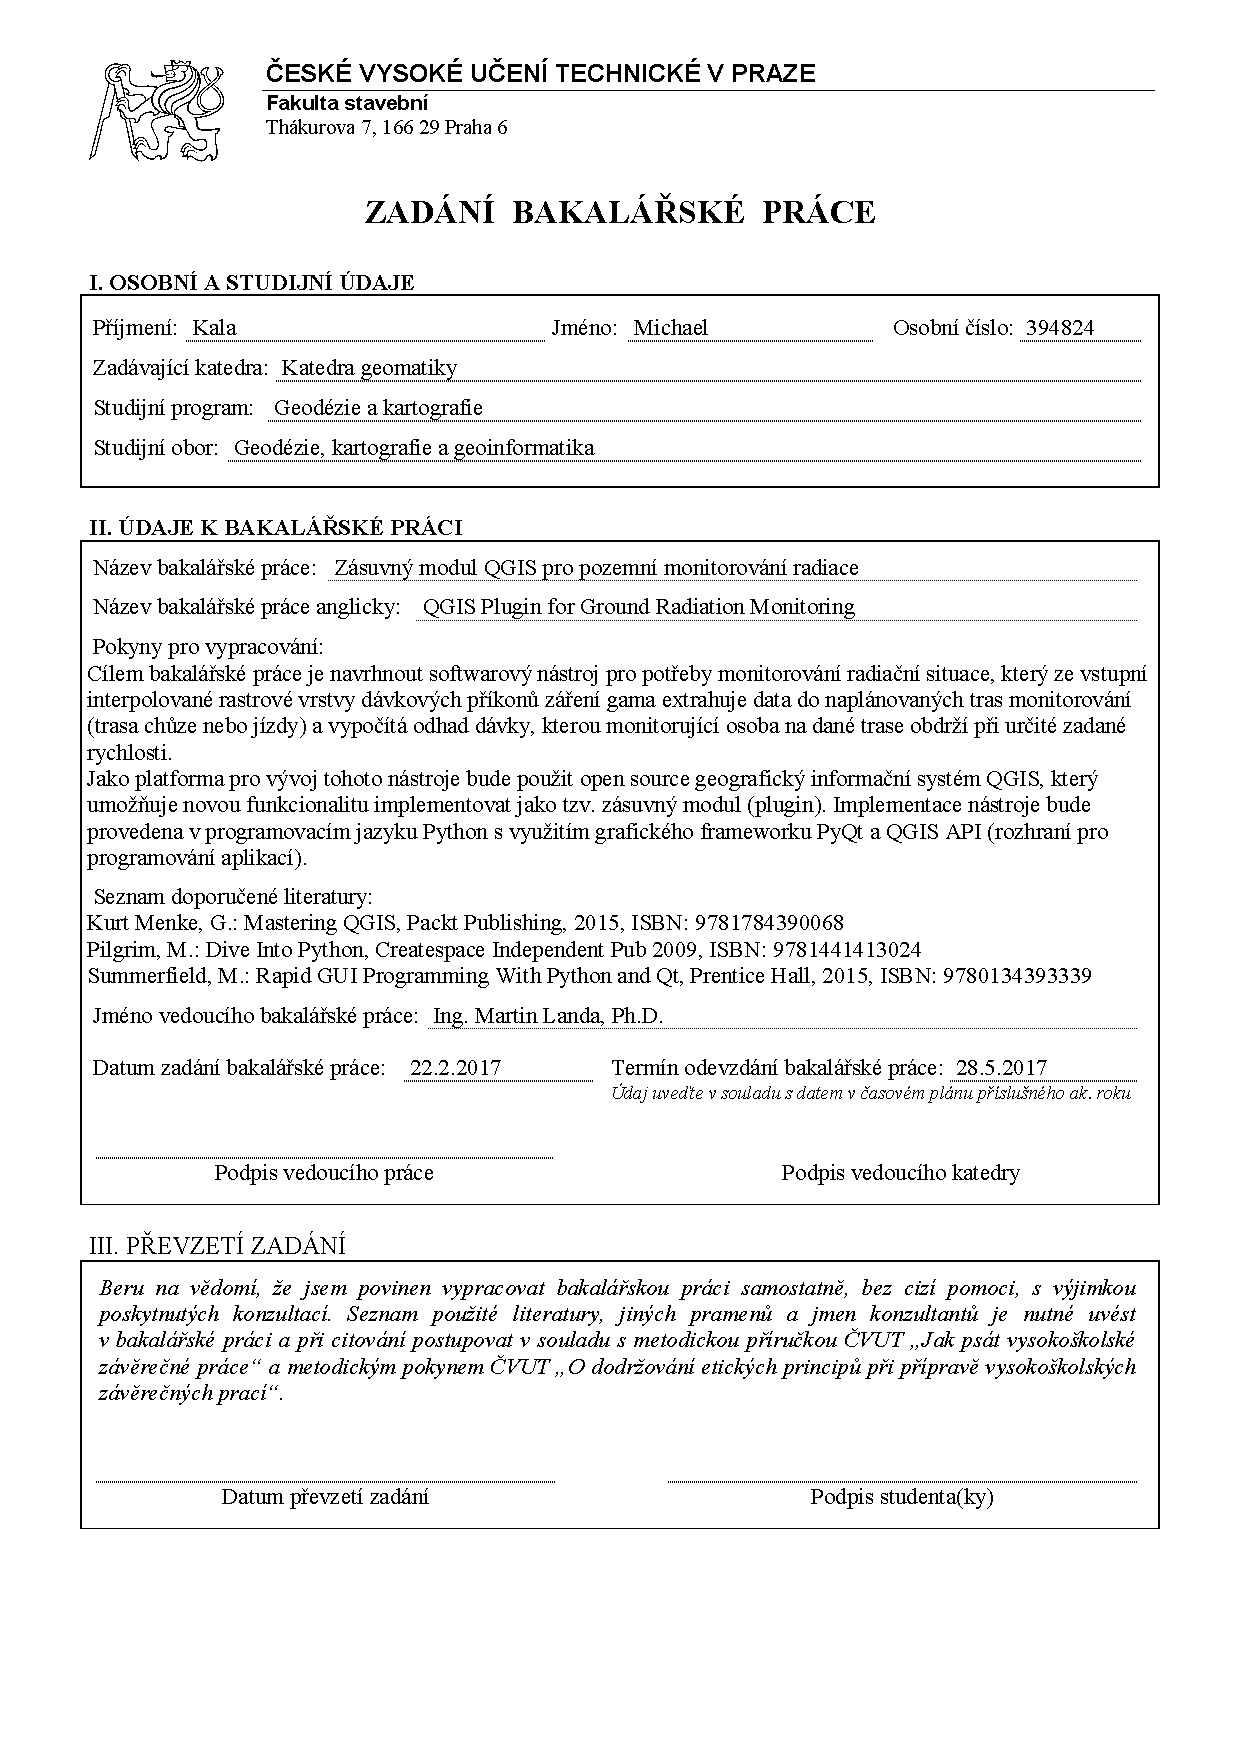
\includegraphics[scale=0.7]{./pictures/zadani.pdf}}%\sffamily\Huge\centering\ }%ZDE VLOŽIT LIST ZADÁNÍ}%
	%{\sffamily\centering Z~důvodu správného číslování stránek}

% Vysázení stránky s abstraktem
\vytvorabstrakt

% Vysázení prohlaseni o samostatnosti
\vytvorprohlaseni

% Vysázení poděkování
\stranka{%nahore
       }{%uprostred
       }{%dole
       \sffamily
	\begin{flushleft}
		\large
		\MakeUppercase{Poděkování}
	\end{flushleft}
	\vspace{1em}
		%\noindent
	\par\hspace{2ex}
	{Rád bych poděkoval Velkému třesku za vznik vesmíru
          z~nekonečně husté singularity, díky čemuž vznikl i život,
          já a tato práce. Také bych se nedokázal obejít bez své
          rodiny a~blízkých, díky kterým jsem v~posledních měsících
          nemusel trávit večery sám s~myšlenkami o~mém
          počínání. Největší díky bych chtěl věnovat mému vedoucímu
          práce Ing. Martinu Landovi Ph.D. za to, že mě na rozdíl od
          přátel k~práci velmi motivoval a příkladně jí vedl. Nakonec
          bych rád poděkoval Mgr. Janu Helebrantovi (SÚRO) za cenné
          připomínky a vždy bleskové odpovědi na mé dotazy.}  }

% Vysázení obsahu
\obsah

% Vysázení seznamu obrázků
\seznamobrazku

% Vysázení seznamu tabulek
\seznamtabulek

% jednotlivé kapitoly
\chapter{Úvod}
\label{1-uvod}
Měření veličin charakterizujících ionizující záření a studium jeho negativních dopadů, jakožto jedna z náplní práce Státního ústavu radiační ochrany, v.v.i. (\zk{SÚRO}), probíhá za účelem ochrany osob a~životního prostředí. 
Hlavní systém zjišťující radiační situaci na území České republiky se nazývá Radiační monitorovací síť (RMS). Vedle Sítě včasného zjištění (SVZ), teritoriální sítě TLD apod. jsou jednou z jejích hlavních složek také mobilní skupiny (MS) provádející pozemní monitorování radiace. \cite{suroRMS}

Cílem této bakalářské práce je implementace softwarového nástroje umožňujícího plánování optimálních tras pozemního monitorování radiace. Při únicích radioaktivních látek do ovzduší je specializovanými softwary spočtena prognóza šíření radioaktivního mraku. Jedním z produktů je také mapa dávkových příkonů záření gama pro zasaženou oblast. Vytvářený softwarový nástroj určí přibližný odhad dávky záření, kterou obdrží mobilní skupina provádějící měření na dané trase v~postiženém území. V případě překročení hraničních hodnot nástroj pomůže v~přeplánování trasy přes jiné komunikace příp. změny rychlosti jízdy vozidla tak, aby mobilní skupina nebyla vystavována nebezpečným dávkám. 
Nástroj může být hypoteticky využit také například pro havarijní plánování při navrhování tras evakuace obyvatelstva. V rámci práce je tvořena offline varianta nástroje nezbytná v případě mimořádných událostí (typu havárie jaderných elektráren), kdy nemusí být k dispozici připojení k internetu. Nicméně v budoucnu by do nástroje mohl také být implementován vlastní online plánovač tras. 

Mimo popisu vývoje nástroje se tato práce bude věnovat teoretickému základu ionizujícího záření, fyzikálním jednotkám, ve kterých je záření měřeno a počítáno, jeho biologickým účinkům na lidský organismus a metodám využívaných mobilními skupinami při pozemním monitorování. 

Nástroj je vytvářen pro \zk{SÚRO}, jako platforma pro vývoj je použit open source geografický informační systém QGIS umožňující implementaci nové funkcionality jako tzv. zásuvný modul (plugin). Nástroj je vyvíjen v programovacím jazyku Python s využitím grafického frameworku PyQt a QGIS API (rozhraní pro programování aplikací).    







\chapter{Teoretický základ}
\label{2-teorie} Tato kapitola se zabývá základy ionizujícího záření,
jeho zdroji a biologickými účinky. Dále je popsána činnost mobilních
skupin provádějících pozemní monitorování radiace. Poslední část
kapitoly stručně pojednává o~přínosu této bakalářské práce a~tvoří
přechod mezi teoretickou a~praktickou částí.

\section{Ionizující záření}
	
Záření (radiace) je proces, při kterém energie prochází
prostorem. Typickými pří\-klady záření, se kterými se setkáváme na denní
bázi, je sluneční svit, rádiový, televizní nebo i wifi signál.

Ionizující záření je záření s~takovým množstvím energie, že může
vyrážet elektrony z~atomového obalu a tím látku ionizovat. Tento jev
se využívá například v~radiologii, lékařském oboru, který ionizující
záření používá za účelem diagnóz, terapií a rozvoje vědy. \citep{who}

\subsection{Druhy ionizujícího záření} Ionizující záření se dělí na
dva druhy: \cite{ionZarUllman} \cite{CEZ}

\begin{itemize}
	\item \textbf{Přímo ionizující}
	
		Kvanta přímo ionizujícího záření nesou elektrický
náboj a přímo vyrážejí elektrony z~atomů. Součástí této kategorie je
např. záření $\alpha$ (prudce letící kladná jádra izotopu helia
$_{2}He^{4}$), $\beta^{-}$ (proud elektronů vznikající při přeměně
neutronu na proton), $\beta^{+}$ (proud kladných pozitronů, antičástic
k~elektronům) atd.
		 
	\item \textbf{Nepřímo ionizující}
	
		Nepřímo ionizující záření předává svou kinetickou
energii nabitým látkovým částicím, které pak látku ionizují. Kvanta
tohoto záření tedy nejsou elektricky nabita. Do této kategorie se řadí
především rentgenové a $\gamma$ záření (elektromagnetická záření
s~velmi nízkou vlnovou délkou).
\end{itemize}

\subsection{Fyzikální jednotky} V~jaderné fyzice se jako základní
jednotka používá becquerel [Bq] patřící mezi odvozené jednotky
soustavy SI. Vyjadřuje střední počet radioaktivních přeměn za
sekundu. Tato jednotka ovšem neříká nic o~druhu záření, jeho
biologickém účinku, energii atd. Pro popis ionizujícího záření jsou
zavedeny veličiny, které slouží jako charakteristiky jeho účinků na
různé látky. \cite{atomInfo}

\begin{itemize}
	\item \textbf{Dávka, dávkový příkon}
	
		 Nejdůležitější z~těchto veličin je tzv. dávka, která
má za jednotku gray [Gy] patřící mezi jednotky SI. Fyzikální
rozměr jednotky gray je joule na kilogram [J/kg]. Častá veličina je
 tzv. dávkový příkon, tedy přírůstek dávky v~čase [Gy/s].
		
	\item \textbf{Ekvivalentní dávka, ekvivalentní dávkový příkon}

	 	V~předchozím bodě zmíněné veličiny nezohledňují
všechny účinky působení záření na živou hmotu. Proto byly zavedeny
radiobiologické veličiny. Patří sem ekvivalentní dávka, která je
vypočtena z~dávky přenásobené tzv. jakostním činitelem Q závisejícím
na typu a energii záření. Hodnota Q je doporučovaná mezinárodní komisí
radiologické ochrany\footnote{V dokumentu ICRP Publication 103
dostupném na
\url{http://www.sujb.cz/fileadmin/sujb/docs/radiacni-ochrana/ICRP103\_dokument.pdf}}. Například
u~gama záření je Q = 1. Ekvivalentní dávka má za jednotku sievert
[Sv], ekvivalentní dávkový příkon pak sievert za jednotku času [Sv/s].
	 	
	\item \textbf{Shrnutí jednotek}
	
		\begin{table}[h!]  \centering
			\caption{Fyzikální jednotky ionizujícího
záření}
			\label{tab:tabulkaJednotek}
			\begin{tabular}{|c|c|c|} \hline \textbf{Název}
& \textbf{Jednotka} & \textbf{Značení} \\ \hline Dávka & gray &
{[}Gy{]} \\ \hline Dávkový příkon & gray za sekundu & {[}Gy/s{]} \\
\hline Ekvivalentní dávka & sievert & {[}Sv{]} \\ \hline Ekvivalentní
dávkový příkon & sievert za sekundu & {[}Sv/s{]} \\ \hline
			\end{tabular}
		\end{table}
\end{itemize}

\subsection{Zdroje ionizujícího záření} Zdroje ionizujícího záření
mohou být přírodní a umělé. Největší ozáření obyvatelstva způsobují
zdroje přírodní, přestože pozornost je věnována především zdrojům
umělým. \cite{radiobiologie}

\begin{itemize}
	\item \textbf{Přírodní zdroje záření}
	
			Tyto zdroje tvoří tzv. přírodní
pozadí. Přírodní zdroje jsou dále rozděleny na dvě kategorie, kosmické
záření a přírodní radionuklidy.  Množství kosmického záření se odvíjí
od nadmořské výšky a zeměpisné šířky kvůli působení zemského
magne\-tického pole na dráhu nabitých částic. Například mezi 30$^{o}$ a
60$^{o}$ jižní resp. severní šířky je intenzita záření příbližně
o~10\% vyšší než na rovníku a magnetických pólech.  Zdroje přírodních
radionuklidů jsou především horniny. Intenzita záření se odvíjí od
původů jednotlivých hornin. Pro ilustraci, vyvřelé horniny vykazují
vyšší aktivitu než horniny metamorfované.
	
	\item \textbf{Umělé zdroje záření}
	
			Za umělé zdroje záření jsou považovány takové
zdroje, které způsobují ozáření při činnostech s~nimi, dále takové
zdroje, které souvisí s~lékařskými zákroky. Běžně se vedle lékařského
ozáření další zdroje podílí na ozáření člověka pouze
minimálně. Dalšími zdroji jsou radionuklidy nacházející se v~životním
prostředí pocházející ze spadu po mimořádných jaderných haváriích
(poškození jaderného zařízení) nebo po zkouškách jaderných
zbraní. Radionuklidy, které se dostaly do ovzduší, se dostávají na
povrch ve formě suchého nebo mokrého spadu s~deštěm, kde kontaminují
vodu a potravu.
			
\end{itemize}

Podrobnější popis zdrojů ionizujícího záření by byl nad rámec této
bakalářské práce, proto nebude dále rozebírán.

\subsection{Biologické účinky ionizujícího záření} Pro stanovení
kritérií a principů radiační ochrany obyvatelstva a pracujících, kteří
přicházejí se zdroji ionizujícího záření více do kontaktu, je potřeba
vědět, jak ioni\-zující záření působí na lidský organismus. Z~těchto
kritérií je dále odvozen systém limitování dávek (viz. kapitola
\ref{sub:limity}). \cite{sujbBiologickeUcinky}

Jak již bylo stručně popsáno, ionizující záření (radiace) způsobuje
ionizaci atomů. Ta může dále vést k~chemickým reakcím, fyzikálním
změnám a v~případě živých tkání k~biochemickým změnám. Tyto změny
mohou vést k~poškození organismu nebo~i~k~jeho úmrtí. Účinek radiace
na organismus je rozdělen na 4 následující etapy: \cite{bioZarUllman}
\newpage
\begin{enumerate}
	\item \textbf{Fyzikální stádium}
	
		Fyzikální stádium je primární proces, při kterém
dochází k~ionizaci atomů (což vede k~narušení chemických vazeb mezi
atomy a molekulami). Při dávce 1Gy se v~objemu každé ozářené buňky
o~typické velikosti 10$\mu$m vytváří 10$^5$ ionizací. Tento proces
trvá jen cca 10$^{-16}$ - 10$^{-14}$s.
		
	\item \textbf{Fyzikálně-chemické stádium}
	
	Sekundárním procesem je fyzikálně-chemické stádium, při kterém
dochází k~disociaci molekul (rozklad na kladně a záporně nabité
částice) a vzniku volných radikálů (vysoce reaktivních částic). Tento
proces je podobně jako proces předchozí velmi rychlý. Trvá přibližně
10$^{-14}$ - 10$^{-10}$s.
	
	\item \textbf{Chemické stádium}
	
	Produkty předchozích stádií reagují s~důležitými organickými
molekulami a mění jejich složení a funkci. Například zlomy řetězců
v~molekule DNA jsou řazeny mezi typické poruchy. Trvání tohoto stádia
ovlivňuje transportní doba reaktivních složek z~místa svého vzniku do
místa napadené biomolekuly v~rozmezí od tisícin sekundy do řádově
jednotek sekund.
	
	\item \textbf{Biologické stádium}
	
	Popsané molekulární změny mohou vyústit ve funkční a
morfologické změny v~buňkách, orgánech a poté i celkově
v~organismu. Trvání této fáze se pohybuje od jednotek sekund (buňky)
až po několik let (organismus). Kdy se biologické stádium projeví,
záleží na množství dávky záření. Při nízkých dávkách se může projevit
až za několik desítek let, kdežto naopak při vysokých dávkách již
během desítek minut.
\end{enumerate}

Lidský organismus má omezenou schopnost opravy poškozených molekul
buněk. Pokud však dávka překročí určitou mez, buňky uhynou a vzniká
tzv. nemoc z~ozáření.


Nemoc z~ozáření může být rozdělena na 2 kategorie: \cite{nemoc}

\begin{itemize}
	\item \textbf{Akutní nemoc z~ozáření}
	
		Akutní nemoc z~ozáření je způsobena jednorázovým
ozářením. Prvotními pří\-znaky jsou nevolnost, zvracení a průjmy. Pokud
dávka ozáření překročí hodnotu přibližně 4 Sv, nastupuje tzv. střevní
forma, kterou doprovází krvavé průjmy a mine\-rální rozvrat. Poté
přichází období latence (prodlevy), jehož délka trvání závisí na
množství absorbované dávky. Po uplynutí latentní fáze nastupuje
tzv. dřeňová forma, kdy dojde k~zhroucení krvetvorby a imunitních
mechanismů. Nemoc v~této fázi dále způsobuje sepsi, sterilitu,
u~těhotných žen potrat atp. Pokud dojde k~absorpci dávek záření
vyšších než 10 Sv, dochází k~nevratnému poškození buněk centrálního
nervového systému a později nastává smrt.
		
	\item \textbf{Chronická nemoc z~ozáření}
	
		Tato forma nemoci z~ozáření se rozvíjí při dlouhodobém
působení malých dávek ionizujícího záření. Dále se dělí na 3
fáze. První z~nich je fáze nespecifických obtíží způsobující
nespavost, bolesti hlavy, pokles počtu bílých krvinek, zažívací obtíže
atd. Další z~fází je fáze výrazné symptomatologie, kde se stupňují
bolesti hlavy, dochází k~poruchám motoriky, k~chronickým průjmům,
váhovým úbytkům atd. Dochází k~poškození centrálního nervového
systému, což doprovází zhoršený sluch a zrak. Následuje poslední fáze
nezvratného poškození. Přestávají fungovat rozmnožovací orgány,
dochází k~poškození srdce, ledvin, jater, dále se na kůži a~sliznici
tvoří vředy atd.

\end{itemize}

\section{Radiační ochrana} Cílem radiační ochrany je zajistit ochranu
obyvatelstva před účinky ionizujícího záření a zároveň umožnit
z~těchto účinků vytěžit co největší přínos (v~radiologii, v~jaderné
energetice atp.). Důležitou součástí radiační ochrany je monitorování
radiační situace. Nasbíraná data slouží pro posuzování stavu ozáření,
pro další potřeby sledování a pro rozhodování o~opatřeních v~případě
radiačních havárií. \cite{suroRadOch} \cite{sujbRadSit}

\subsection{Limity expozice ionizujícímu záření v~České republice}
\label{sub:limity} Stupeň povoleného ozáření obyvatelstva se řídí
omezeními, která jsou určována le\-gislativou ve vyhláškách úřadů
zabývajících se touto problematikou (\zk{SÚRO}, \zk{SÚJB}). Konkrétně
pro Českou republiku je to vyhláška 307/2002 Sb. Na základě doporučení
pracovníků SÚRO jsou hodnoty dávky resp. dávkového příkonu udávané
v~jednotkách microsievert [$\mu$Sv] resp. microsievert za hodinu
[$\mu$Sv/h]. Limity expozice ionizujícímu záření v~ČR jsou patrné
z~obrázku \ref{fig:davkyCR}. \cite{suroPriRadOch}

\begin{figure}[H] \centering
    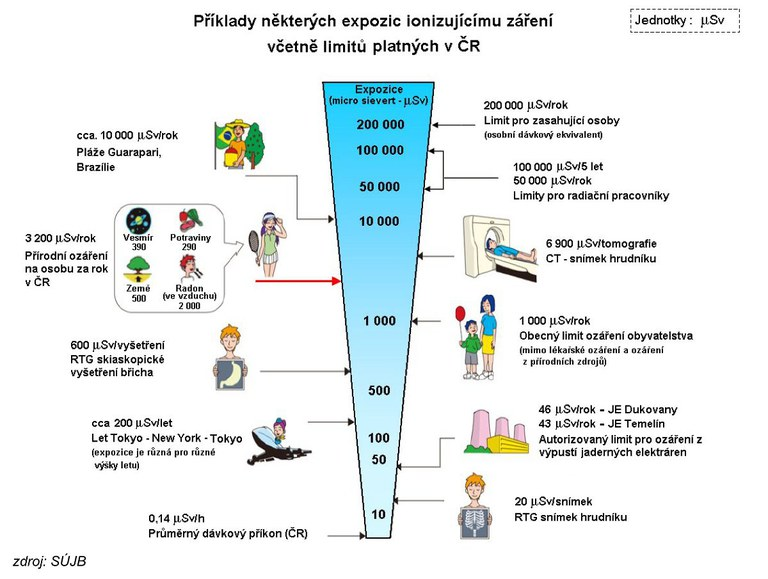
\includegraphics[scale=0.6]{./pictures/davkyCR.jpeg}
      	\caption[Příklady expozice a limity]{Příklady expozice a
limity (zdroj: \cite{suroOcek})}
    	\label{fig:davkyCR}
\end{figure}

\subsection{Pozemní monitorování radiační situace} Pomocí
tzv. Radiační monitorovací sítě (\zk{RMS}) je zjišťována radiační
situace na území České republiky. Na činnosti \zk{RMS} se podílejí
resorty různých ministerstev (financí, obrany, vnitra atd.), dále
držitelé povolení k~provozu jaderných zařízení a~hlavně Státní ústav
radiační ochrany (\zk{SÚRO}). Řízením je pověřen Státní ústav pro
jadernou bezpečnost (\zk{SÚJB}). \cite{suroRMS}

Součástí \zk{RMS} jsou i mobilní skupiny (\zk{MS}), jejichž úkolem je
dodat krizovému štábu při radiačních haváriích (radiační nehoda
vyžadující opatření na ochranu obyvatelstva a životního prostředí)
dostatek dat pro posouzení radiační situace a návrh nutných
opatření. \zk{MS} při jízdě autem kontinuálně monitorují ekvivalentní
dávky resp. ekvivalentní dávkové příkony (pro zjednodušení dále
v~textu jako dávky resp. dávkové příkony), odebírají vzorky složek
životního prostředí atd.  \cite{metodika} \cite{pecha2011monitorovani}

\begin{figure}[H] \centering
    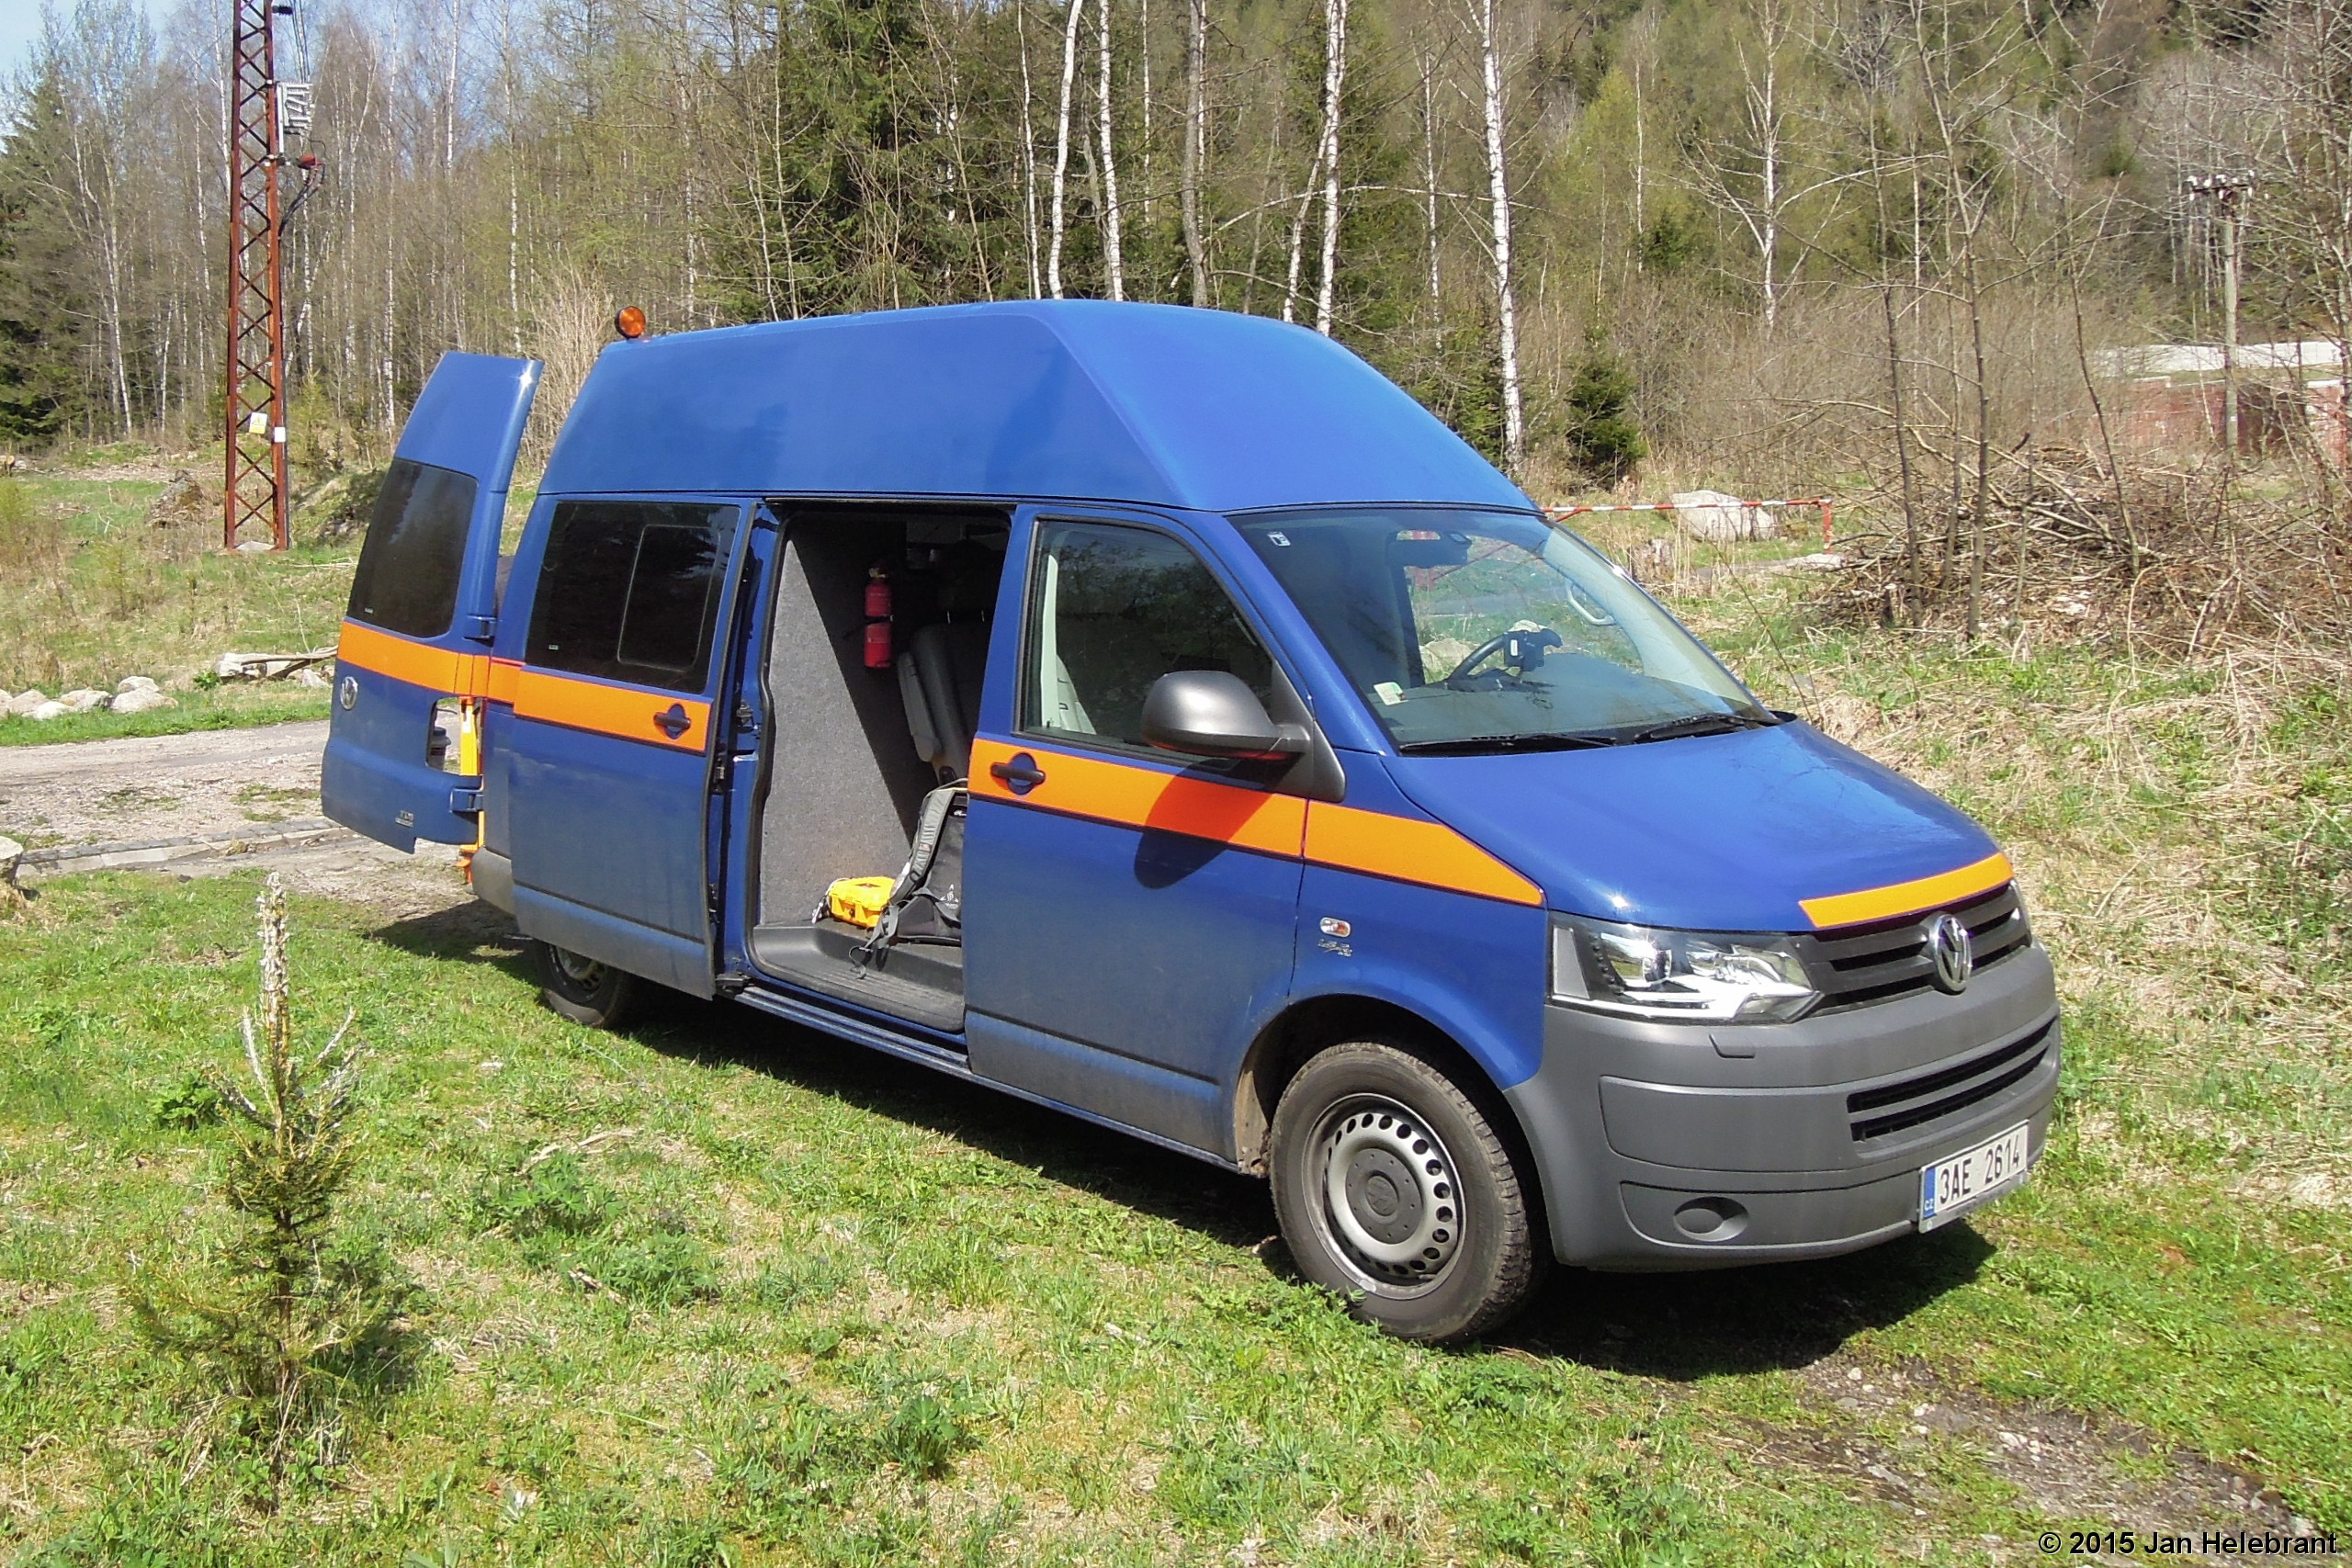
\includegraphics[scale=0.6]{./pictures/vuzSURO.jpg}
      	\caption[Vůz \zk{MS} \zk{SÚRO} Praha]{Vůz \zk{MS} \zk{SÚRO}
Praha (zdroj: SÚRO, v.v.i.)}
    	\label{fig:vuzSURO}
\end{figure}

Před vlastním únikem škodlivých látek do ovzduší při radiačních
haváriích jsou k~dispozici modelové prognózy vznikající radiační
události získané na základě napočítaných havarijních sekvencí,
reálných údajů a meteorologické situace. Vedle těchto modelů jsou již
v~době úniku měřeny hodnoty dávkových příkonů ze sítě dozimetrů
(zařízení k~měření dávek ionizujícího záření) rozmístěných
po areálu jaderné elektrárny. Všechny tyto informace napomáhají
krizovému štábu identifikovat směr úniku a vytipovat oblasti
monitoringu pro \zk{MS}.

\subsubsection{Fáze radiační havárie}

Radiační havárie v~jaderné elektrárně (a její řešení) je rozdělena na
3 hlavní fáze:

\begin{itemize}
	\item \textbf{Časná fáze}
	
		Časná fáze zahrnuje dobu přibližně 1-2 dnů po ukončení
úniku látek z~havarované jaderné elektrárny. Během této fáze je nutné
co nejdříve zmapovat dávkové příkony na daném území. Pro lepší
komunikaci mezi krizovým štábem a \zk{MS} jsou předpřipravené trasy,
které jsou dále upravovány podle naměřených hodnot. Blízké okolí
jaderných elektráren (20km JE Dukovany, 13km JE Temelín) je rozděleno
na 16 sektorů. V~každém sektoru je právě pro prvotní fázi monitorování
připravena 1 trasa monitorování zasahující i do sektorů
vedlejších. Vytipována je ještě 17. pojezdová trasa, která je vedena
po blízkém okolí jaderné elektrárny. Cílem časné fáze je pomocí
měřených hodnot v~daném místě a čase upřesnit modelovou prognózu a
získat tak podklady pro rozhodování o~evakuaci obyvatelstva.

	\item \textbf{Střední a pozdní fáze}
		
		Střední a pozdní fáze může mít v~závislosti na
závažnosti havárie trvání několik týdnů až roků. Tato fáze má za cíl
získat podklady k~rozhodnutí o~dalších ochranných opatřeních, ukončení
evakuace, regulaci potravních řetězců, přesídlení obyvatelstva
z~kontaminované oblasti atp. Úkolem \zk{MS} je vedle detailnějšího
pojezdového monitorování sběr vzorků životního prostředí a jejich
předání do specializovaných laboratoří pro analýzy. Dále je to na
základě měření leteckých skupin, které vyhledávají tzv. horká místa
(místa s~významně vyšším dávkovým příkonem), upřesňování výsledků
těchto měření.
\end{itemize}

\subsubsection{Havarijní připravenost}

Obzvlášť pro časnou fázi radiační havárie je třeba, aby byly
připravené a nacvičené postupy a metodiky, podle kterých se \zk{MS}
mají řídit. Kvůli připravenosti probíhají havarijní cvičení pořádaná
\zk{SÚJB}, kde jsou procvičeny všechny postupy. Tyto nácviky probíhají
měsíčně, kdy každá \zk{MS} projede trasu dlouhou cca. 40km, naměří
dávkové příkony a vloží je do databáze. Jednou za čas také probíhají
cvičení ve větším měřítku (cvičení ZÓNA), kdy jsou simulovány radiační
havárie. Zapojovány jsou všechny složky, které by byly zapojeny během
skutečné havárie. Poslední takové cvičení proběhlo v~roce 2017, kdy
byla simulována havárie v~jaderné elektrárně Dukovany.

\subsubsection{Bezpečnost práce}

Členové \zk{MS} se účastní měření v~souladu se zásadami bezpečnosti a
ochrany zdraví, které jsou stanoveny příslušnými zákony a vyhláškami
(např. zákon č.309/2006 Sb. - zákon o~zajištění dalších podmínek
bezpečnosti a ochrany zdraví při práci). Pracovníci používají při
výjezdech osobní ochranné pomůcky (ochranný oděv, pracovní obuv,
respirátor atd.) a dále jsou vybaveni osobními dozimetry.

%%% ML: Nepatri tato zasadni kapitola spise do zaveru?
%%% MK: Přesunul jsem

\chapter{Použité technologie}
\label{3-technologie}

Tato kapitola rozebírá technologie použité pro tvorbu nástroje.
\section{QGIS}

\begin{figure}[H]
    \centering
      
\includegraphics[width=100pt]{./pictures/qgis.png}
      \caption[QGIS logo]{QGIS logo}(zdroj: %https://commons.wikimedia.org/wiki/File:QGis_Logo.png)
      \label{fig:qgis}
  \end{figure}
 
% http://docs.qgis.org/2.14/en/docs/user_manual/preamble/foreword.html
QGIS je multiplatformní geografický informační systém (\zk{GIS}) vyvíjený jako Open Source šířený pod Obecnou veřejnou licencí GNU (\zk{GNU GPL}). \zk{GNU GPL} zaručuje svobodu jeho sdílení a úprav, které vedou k implementaci nových funkcionalit a k jeho zdokonalení. To z něj činí mocný nástroj používaný ve veřejném i soukromém sektoru. QGIS je psán v programovacím jazyku C++, jeho grafické uživatelské rozhraní je postaveno na knihovně Qt. Projekt QGIS započal v roce 2002, verze 1.0 byla uveřejněna roku 2009. 

QGIS disponuje nepřeberným množstvím zásuvných modulů (pluginů) rozšiřujících funkčnost softwaru. Pluginy jsou programovány v jazyku C++ nebo Python. 

Open source nutně neznmná nepodporovný, právě naopak, velikost on-line komunity zabývající se QGIS a její rychla odezva...



\section{Python}
\begin{figure}[H]
    \centering
      
\includegraphics[width=100pt]{./pictures/python.png}
      \caption[Python logo]{Python logo}(zdroj: %???)
      \label{fig:python}
  \end{figure}
  
Python je objektově orientovaným skriptovacím jazykem zkompilovatelným téměr na každé platformě. Oceňován programátory (především začátečníky) je pro svou jednoduchou a velice schopnou syntax, například také díky dynamickému typování (nepožaduje specifikaci datového typu u proměnných). Dále jeho objektový model podporuje polymorfismus, přetěžování operátorů a vícenásobnou dědičnost. Hlavním důvodem, proč je zařazován mezi skriptovací jazyky je jeho integrace s jazykem C. Díky knihovnám Python/C API lze z programů v Pythonu volat kód psaný v C nebo naopak, pro aplikace psané v C je možné integrovat interpret Pythonu. %naučte se Python knížka
Python bývá označován jako "spustitelný pseudokód" - syntaxe se snaží vyhnout složitým zápisům a znakům ($\$, <<, \&\&, ?$), inspiruje se v matematice zápisem abstraktních algoritmů.%http://naucse.python.cz/lessons/intro/magic/

Jazyk Python byl navržen koncem 80. let nizozemským počítačovým programátorem Guido van Rossumem. První verzi (0.9.0) uveřejnil začátkem roku 1991. Hlavní principy Pythonu, které zakladatel jazyka prosazuje, byly shrnuty do podoby 20 aforismů (\textit{"Zen of Python, by Tim Peters"}), např.:

\begin{itemize}

	\item
		\textit{Na čitelnosti záleží. (Readability counts.)} 	
			
	\item
		\textit{Chyby by nikdy neměly projít bez povšimnutí. Jedině pokud nejsou záměrně zamlčeny. (Errors should never pass silently. Unless explicitly silenced.)}
		
	\item
		\textit{Měl by existovat jeden - a pokud možno pouze jeden - zřejmý způsob jak to udělat. (There should be one - and preferably only one - obvious way to do it.)}
\end{itemize}  

Pro výpis anglického originálu Zenu stačí do konzole Pythonu napsat \\ \texttt{$>>>$~\textbf{import}~this}. Od roku 2008 je vyvíjena řada Pythonu 3, která se snaží naplnit právě poslední ze zmiňovaných aforismů, kdy důraz je kladen na odstranění duplicitních programových konstrukcí a modulů. Python 3 není plně zpětně kompatibilní s řadou 2, softwary napsané a využívající Python 2 postupně přecházejí na jeho novou verzi (i QGIS s připravovanou verzí QGIS 3.0). Pro zajímavost, jazyk byl pojmenován podle britské komediální skupiny Monty Python.  %http://www.python-course.eu/python3_history_and_philosophy.php


\section{Qt}


%%% ML: poznamce pod carou v nazvu kapitoly by bylo dobre se vyhnout
%%% (ikonku premistit dal do textu a pod)
\chapter[Zásuvný modul]{Zásuvný
modul 
\includegraphics[scale=0.65]{./pictures/ikonka.png}\footnote{Zdroj:
SÚRO, v.v.i.}}
\label{4-plugin}

V~následujícím textu bude popsán postup tvorby nového softwarového
nástroje \textit{Ground radiation monitoring} a jeho
funkcionalita. Při vývoji nástroje bylo čerpáno z~doporučené
literatury \cite{masteringQgis} \cite{diveIntoPython} \cite{rapidPyQt}.

\section{Zadání} Zadáním bakalářské práce bylo vytvoření softwarového
nástroje, který ze vstupní interpolované mapy dávkových příkonů
extrahuje data do naplánovaných tras moni\-torování a vypočítá obdrženou
dávku záření gama při zadané rychlosti. Nástroj dále vypočte
jednoduché statistiky, maximální a průměrný dávkový příkon, délku
trasy, čas a kumulativní dávku v~určitých zadaných intervalech.

\subsection{Vstupní data}
\label{subsec:vstupniData}
\begin{enumerate}
	\item \textbf{Interpolovaná mapa dávkového příkonu} \\ Mapa je
v~souřadnicovém systému WGS84 EPSG:4326. Je vytvořena v~rastrovém
formátu, který je podporován knihovnou
GDAL\footnote{\url{http://www.gdal.org/formats\_list.html}}. Obsahuje
hodnoty dávkového příkonu v~daných jednotkách. (Plugin umožňuje volit
typ jednotek).
	\item \textbf{Trasa monitorování} \\ Trasa monitorování je
taktéž v~souřadnicovém systému WGS84 EPSG:4326. Je vytvořena ve
vektorovém formátu, který je podporován knihovnou
OGR\footnote{\url{http://www.gdal.org/ogr\_formats.html}}. Trasy mohou být
generované pomocí plánovačů tras (např. společnosti Google, Inc.)
\end{enumerate}

\begin{figure}[H] \centering
    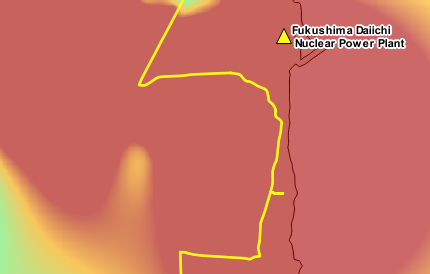
\includegraphics[scale=0.6]{./pictures/ukazka_vstupnich_dat.png}
    \caption[Ukázka vstupních dat]{Ukázka vstupních dat (zdroj:
vlastní, data poskytnutá od SÚRO, v.v.i.)}
    \label{fig:vstup}
\end{figure}
  			
\subsection{Výstupní data}
\label{sec:VystupniData}
\begin{enumerate}
	\item \textbf{Soubor se zprávou o~výpočtu} \\ Soubor se
zprávou o~výpočtu v~textovém formátu (\textit{.txt}) obsahuje
následující informace o~výpočtu (v~anglickém jazyce):
		\begin{itemize}
			\item čas vytvoření zprávy (\textit{report
created})
			
			\item informace o~trase (\textit{route
information})
			\begin{itemize}
				\item název trasy (\textit{route})
				\item zadaná rychlost v~km/h
(\textit{monitoring speed (km/h)})
				\item celkový čas monitorování
v~h:mm:ss (\textit{total monitoring time (h:mm:ss)})
				\item celková vzdálenost v~km
(\textit{total distance (km)})
			\end{itemize}
			
			\item informace o~části trasy bez dostupných
dat (v~místech, kde trasa přesahuje mapu dávkového příkonu)
(\textit{no data})
			\begin{itemize}
				\item čas (\textit{time})
				\item vzdálenost v~km
(\textit{distance (km)})
			\end{itemize}
			
			\item statistické hodnoty (\textit{radiation
values (estimated)})
			\begin{itemize}
				\item maximální dávkový příkon
v~$\mu$Sv/h (\textit{maximum dose rate ($\mu$Sv/h)})
				\item průměrný dávkový příkon
v~$\mu$Sv/h (\textit{average dose rate ($\mu$Sv/h)})
				\item celková dávka v~$\mu$Sv
(\textit{total dose ($\mu$Sv)})
			\end{itemize}
			
			\item nastavení (\textit{plugin settings})
			\begin{itemize}
				\item jednotky dávkového příkonu
vstupní mapy (\textit{input raster units})
				\item vzdálenost mezi body
navzorkované trasy v~m (vysvětleno v~kapitole
\ref{subsec:vzorkovaniLinie} (\textit{distance between track vertices
(m)})
			\end{itemize}
			
		\end{itemize}
Ukázku zprávy o výpočtu lze nalézt v obrázku \ref{fig:report}.	
			\begin{figure}[H] \centering
      			
\includegraphics[scale=0.9]{./pictures/report.png}
      				\caption[Ukázka zprávy
o~výpočtu]{Ukázka zprávy o~výpočtu (zdroj: vlastní)}
     				\label{fig:report}
  			\end{figure}
  			
	\item \textbf{Soubor trasy} \\ Soubor trasy obsahuje bodovou
vrstvu ve formátu Esri Shapefile (\textit{.shp}) s~body trasy
navzorkované dle zadání uživatele (vysvětleno v~kapitole
\ref{subsec:vzorkovaniLinie}) s~následujícími atributy (obr. \ref{fig:atributova_tabulka})
		\begin{itemize}
			\item dávkový příkon (\textit{rate uSvh})
			\item kumulativní čas (\textit{accTime})
			\item časový interval mezi body (\textit{interval s})
			\item kumulativní dávka (\textit{accDose})
		\end{itemize}
			\begin{figure}[H] \centering
      			
\includegraphics[scale=1]{./pictures/atributova_tabulka.png}
      				\caption[Výřez atributové
tabulky]{Výřez atributové tabulky (zdroj: vlastní)}
     				\label{fig:atributova_tabulka}
  			\end{figure}
  	
  	\item \textbf{Soubor s~údaji o~trase (volitelné)} \\ V~souboru
s~údaji o~trase ve formátu \zk{CSV} (\textit{.csv}) (obr. \ref{fig:csv}) jsou obsaženy
stejné hodnoty jako v~atributové tabulce navzorkované trasy. Navíc
soubor obsahuje souřadnice bodů. Vytvoření souboru je volitelné.
  			\begin{figure}[H] \centering
      			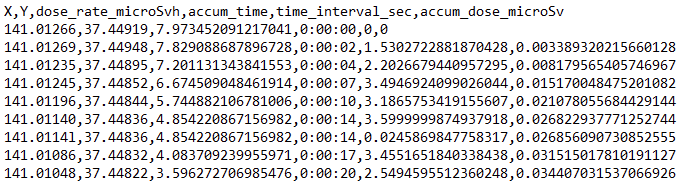
\includegraphics[scale=0.8]{./pictures/csv.png}
      				\caption[Výřez ze souboru s~hodnotami
oddělenými čárkou]{Výřez ze souboru s~hodnotami oddělenými čárkou
(zdroj: vlastní)}
     				\label{fig:csv}
  			\end{figure}
\end{enumerate}

\section{Kostra zásuvného modulu}
\subsection[Plugin Builder]{Plugin
Builder 
\includegraphics[scale=0.1]{./pictures/plugin_builder.png}}
K~vytvoření základu softwarového nástroje byl použit zásuvný modul
Plugin Builder dostupný z~oficiálního QGIS
repozitáře.\footnote{Dostupné
z~\url{https://plugins.qgis.org/plugins/pluginbuilder/}} Tento modul
pochází z~dílny organizace GeoApt LLC, jež se zabývá volně šiřitelnými
GIS. Po zadání základních informací (název modulu, základní popis,
autor, požadovaná verze QGIS, odkazy a další údaje o~repozitáři apod.)
vytvoří Plugin Builder kostru nového zásuvného modulu. Tato kostra
zajišťuje základní funkcionalitu modulu, tedy zobrazení a vypnutí okna
nebo také tlačítka \texttt{OK | Cancel}, pokud okno zásuvného modulu
není nastaveno jako "přichycovací".

\subsection{Popis souborů} Celý zásuvný modul \textit{Ground radiation
monitoring} se skládá z~několika souborů dohromady tvořících balíček,
který zajišťuje spustitelnost a funkcionalitu modulu. Některé soubory
zde budou dále prezentovány. Funkcionalita zásuvného modulu
zajišťující řešení zadání bakalářské práce je implementována v~posledních
dvou souborech následujícího výčtu.

\begin{itemize}
	\item \textbf{\_\_init\_\_.py} \\ Soubor slouží pro základní
inicializaci modulu.
		 
	\item \textbf{metadata.txt} \\ Tento textový soubor obsahuje
informace o~zásuvném modulu čtené Správcem zásuvných modulů. Vedle
údajů jako je jméno autora a název modulu je zde napří\-klad také údaj
o~požadované verzi QGIS, pro kterou je modul naprogramován. Správce
pak tento údaj porovná s~verzí QGIS a pokud dojde ke konfliktu, vypíše
chybovou hlášku a modul nenaimportuje.
	
	\item \textbf{Makefile} \\ V~souboru se nachází set instrukcí
např. pro zkompilování dokumentace nebo souboru \textbf{resources.qrc}
(zkompilovaná verze je \textbf{resources.py}), který informuje Qt jak
naložit s~ikonou modulu.
		
	\item \textbf{plugin\_upload.py} \\ Tento soubor slouží pro
nahrání modulu do QGIS repozitáře zásuvných modulů.

	\item \textbf{ground\_radiation\_monitoring.py} \\ Soubor
slouží pro implementaci zásuvného modulu do prostředí QGIS. Obsahuje
třídu \texttt{GroundRadiationMonitoring}. Zásadními metodami této
třídy jsou \texttt{add\_action} - metoda načítající ikonu modulu
(včetně názvu) do nástrojové lišty QGIS a~do~menu (přidává tedy
tlačítko na spuštění) a dále jsou to metody \texttt{onClosePlugin} a
\texttt{unload}, které se starají o~destrukci modulu.

	\item \textbf{ground\_radiation\_monitoring\_dockwidget.py} \\
Soubor zajišťuje propojení s~grafickým rozhraním, které je vytvořené
v~souboru \textbf{ground\_radiation\_monitoring\_base.ui} pomocí
prostředí QT Designer. Obsahuje třídu
\texttt{GroundRadiationDockWidget}, ve které jsou implementovány metody
pro načítání vstupních dat, čtení údajů zadaných uživatelem a
především také pro spuštění (a případné přerušení) procesu výpočtu a
práci s~výstupním souborem trasy (pokud si to uživatel přeje, vrstva
s~trasou může být načtena do QGIS). V~případě chyby při zadání
vstupních parametrů (např. zadání textu do pole, do kterého má být
zadané číslo nebo výběr výstupního souboru, do kterého je zápis
zakázán) je uživatel upozorněn chybovým hlášením.
	
	\item \textbf{ground\_radiation\_monitoring\_computation.py}
\\ V~souboru probíhá samotný výpočet dle uživatelsky zadaných dat a
vstupních parametrů. Obsahuje třídu
\texttt{GroundRadiationMonitoringComputation}, která je implementována
jako samostatné výpočetní vlákno. Výhodou je, že výpočet probíhá na
pozadí, tedy že s~QGIS se dá pracovat dále nezávisle na probíhajícím
procesu, což je nezbytné vzhledem k~jeho někdy dlouhému trvání
(v~závislosti na vstupních proměnných). V~této třídě jsou vedle
výpočetních metod obsaženy také metody pro vytváření výstupních
souborů. Třída během výpočtu komunikuje s~hlavním vláknem (s~třídou
\texttt{GroundRadiationMonitoringDockWidget}). Přes signály informuje
o~postupu výpočtu, který je zobrazován v~ukazateli průběhu výpočtu.
	
\end{itemize}

\newpage
\section{Algoritmus} V~této části práce bude popsán algoritmus
kódu. Nejprve bude prezentováno jednoduché schéma výpočtu, poté budou
jednotlivé části rozebrány více dopodrobna.
\subsection{Schéma výpočtu}
\begin{figure}[H] \centering
    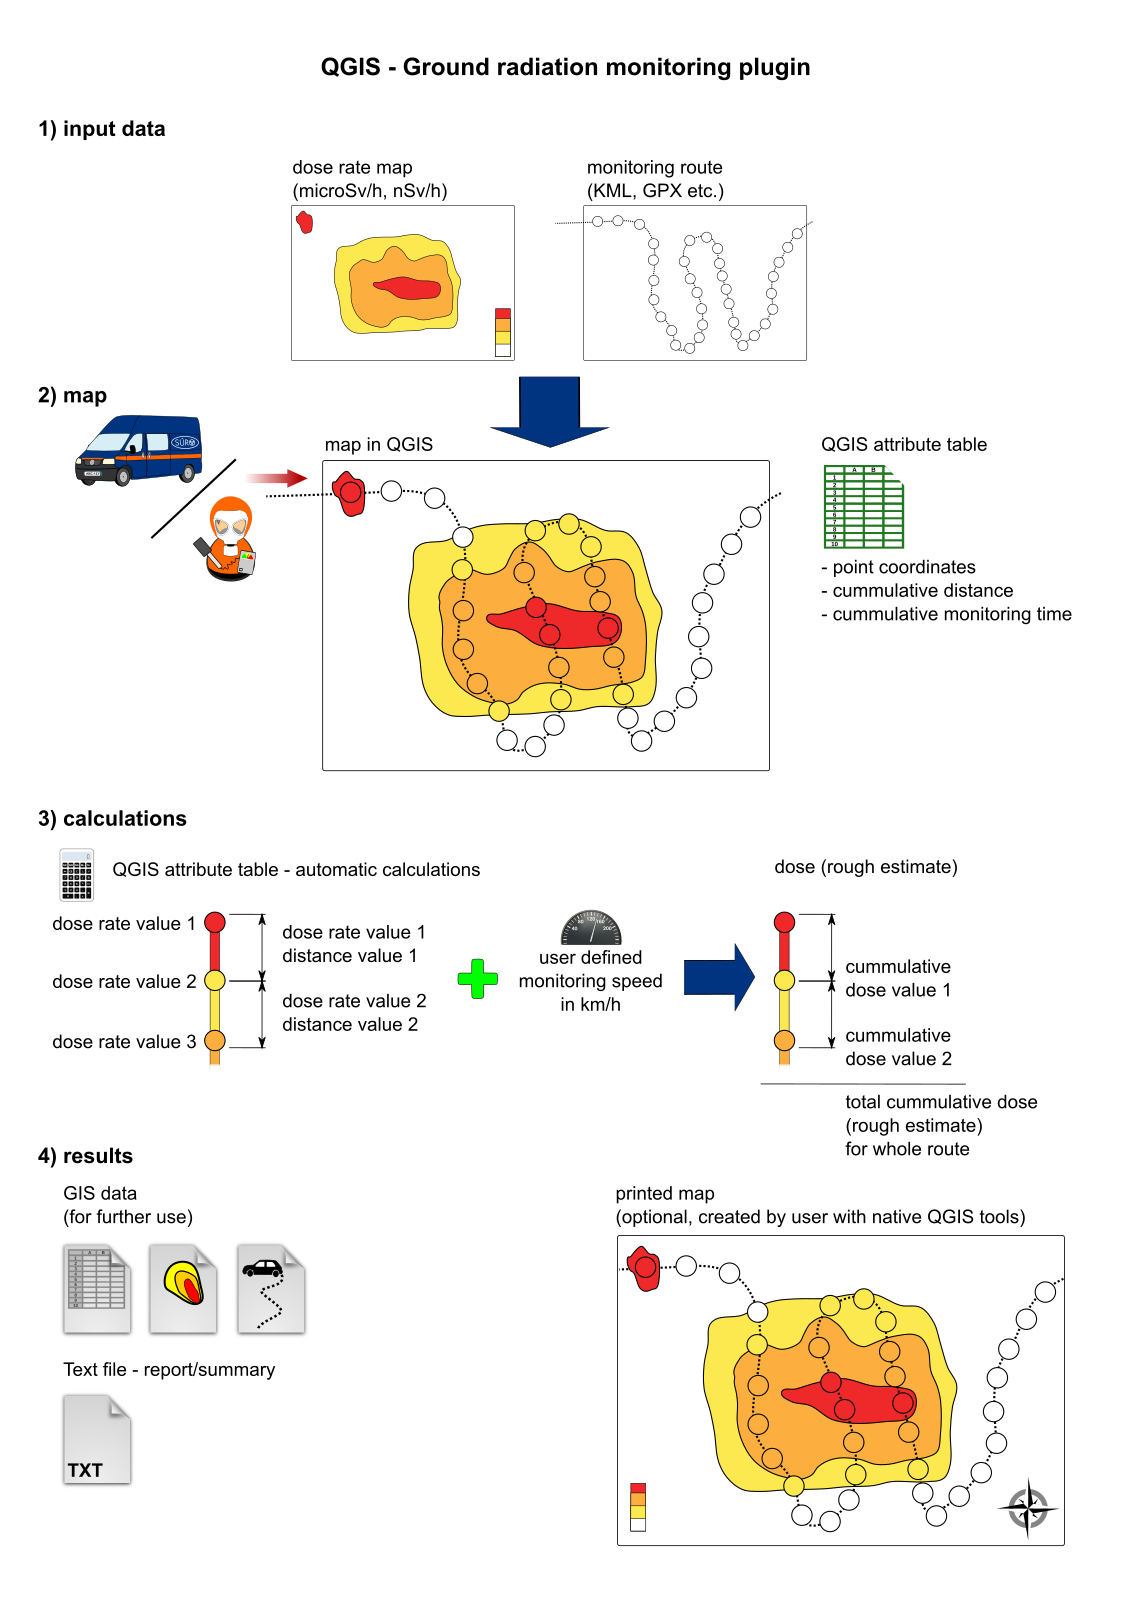
\includegraphics[scale=0.4]{./pictures/computation_scheme.png}
      	\caption[Schéma výpočtu]{Schéma výpočtu (zdroj: SÚRO, v.v.i.)}
    	\label{fig:SchemeOfComputation}
\end{figure}

Schéma výpočtu je zřejmé z~obrázku
\ref{fig:SchemeOfComputation}. Z~interpolované mapy dávkových příkonů
(\textit{dose rate map}) jsou extrahovány rastrové hodnoty
(\textit{dose rate value}) v~bodech navzorkované trasy
(\textit{monitoring route}). Dále jsou provedeny výpočty, tedy dle
vzdálenosti (\textit{distance value}) mezi jednotlivými body trasy a
zadané rychlosti (\textit{user defined monitoring speed}) je spočtena
obdržená dávka záření na daném úseku (\textit{cumullative)}. Rychlost
je konstantní pro celou trasu. Tyto hodnoty společně s~časy potřebnými
na projetí jednotlivých úseků jsou zapsány do atributové tabulky nově
vzniklé vrstvy a volitelně do \zk{CSV} souboru. Statistiky o~celé
trase, jak již bylo řečeno v~sekci \ref{sec:VystupniData}, jsou
uloženy do textového souboru se zprávou o~výpočtu.

\subsection{Vzorkování linie}
\label{subsec:vzorkovaniLinie} Vstupní trasa monitorování se skládá
z~několika přímých linií vzájemně propojených vrcholy. Délka
jednotlivých segmentů se odvíjí od přímosti úseků trasy. Např. pokud
součástí trasy bude dálnice s~přímým úsekem dlouhým 10 km, pak stejně
bude dlouhý i segment mezi vrcholy na začátku a konci tohoto
úseku. Jelikož snímání hodnot rastru probíhá na daných souřadnicích a
jediné známé souřadnice trasy jsou právě ty vrcholové, tak by bez
dalších úprav došlo k~hrubým chybám ve výpočtech resp. výsledky by
byly nesměrodatné. Je jasné, že kdyby uprostřed dlouhého rovného úseku
byla oblast se zvýšeným dávkovým příkonem, tak tato skutečnost by do
výpočtu nebyla vůbec zahrnuta (hodnoty rastru by byly sejmuté pouze na
koncích, tedy v~místech, která nenesou žádnou informaci o~zbytku
segmentu).

Z~tohoto důvodu je třeba trasu tzv. navzorkovat, tzn. rozdělit
jednotlivé rovné segmenty na více kratších částí. Takto dojde
k~získání souřadnic bodů, které mezi sebou budou mít kratší
vzdálenosti. Do výpočtu bude tak zahrnuto více informací o~dávkových
příkonech v~průběhu trasy a výsledek bude lépe odpovídat
skutečnosti. (Stále se však vzhledem k~jednoduchosti výpočtu bude
jednat pouze o~odhad).

Některé segmenty mohou být kratší, než uživatelsky zadaná vzorkovací
vzdálenost. Následující pseudokód
\ref{alg:getTrackVertices} popisuje algoritmus \texttt{Získání
souřadnic bodů trasy} (ve třídě
\texttt{GroundRadiationMonitoringComputation} jako metoda
\texttt{getTrackVertices}), který získává souřadnice vrcholů trasy a
na základě výpočtu vzdálenosti rozhoduje, zdali je potřeba trasu
v~jednotlivých segmentech navzorkovat. Pokud ano, segment je ihned
navzorkován zavoláním \texttt{navzorkujLinii} (ve třídě \\
\texttt{GroundRadiationMonitoringComputation} jako metoda
\texttt{sampleLine}). Výstupem algoritmu pro získání souřadnic je
dvourozměrné pole obsahující souřadnice bodů již navzorkované
linie. Vzdálenost mezi body je vypočtena pomocí QGIS třídy
\texttt{QgsDistanceArea}\footnote{\url{https://qgis.org/api/classQgsDistanceArea.html}}
a jejích metod, výpočet je proveden na referenčním elipsoidu
\textit{WGS84}. Extrahování souřadnic vrcholů trasy je provedeno
pomocí QGIS třídy
\texttt{QgsVectorLayer}\footnote{\url{https://qgis.org/api/classQgsVectorLayer.html}}
a její metody \texttt{getFeatures}.

\begin{algorithm}
\caption{Získání souřadnic bodů trasy}
\label{alg:getTrackVertices}
    \begin{algorithmic}[1] \STATE{\textbf{funkce} získejSouřadnice}
\STATE{extrahuj souřadnice vrcholů trasy do poleSouřadniceVrcholů}
\STATE{přidej poleSouřadniceVrcholů[0] do poleNovéSouřadnice} \FOR{i =
řada od 0 do (délka(poleSouřadniceVrcholů) - 2)} \STATE{bod1 =
poleSouřadniceVrcholů[i]} \STATE{bod2 = poleSouřadniceVrcholů[i + 1]}
\STATE{vzdálenost = vypočtiVzdálenost(bod1, bod2)} \IF{vzdálenost >
vzorkovacíVzdálenost} \STATE{novéBody = navzorkujLinii(bod1, bod2)}
\STATE{přidej novéBody do poleNovéSouřadnice} \ELSE \STATE{přidej bod2
do poleNovéSouřadnice}
    		\ENDIF
    	\ENDFOR \STATE{\textbf{return} poleNovéSouřadnice}
    \end{algorithmic}
\end{algorithm}

Je zřejmé, že všechny nově vzniklé úseky trasy nemají stejnou
délku. Je to dané tím, že délka původních segmentů není většinou
dělitelná zadanou vzorkovací vzdáleností bez zbytku. Např. segment
o~délce 10 m při vzorkovací vzdálenosti 3~m bude rozdělen celkem na
čtyři části, z~toho tři budou o~délce 3~m a jeden o~délce 1
m. Následující pseudokód \ref{alg:sampleLine} popisující výpočetní
funkci souřadnic nových bodů tuto skutečnost zohledňuje a
ověřuje. Algoritmus vypočte souřadnice bodu, který zakončuje tu část
segmentu, která je dělitelná vzorkovací vzdáleností beze zbytku (pokud
nastane případ, že segment je dělitelný beze zbytku, tato část
algoritmu není vykonávána). Tento bod je poté považován za konečný bod
(v~pseudokódu jako \texttt{konečnýBod}) segmentu a nově vzniklý úsek
je rozdělen na stejně dlouhé části.

\begin{algorithm}
\caption{Výpočet souřadnic bodů}
\label{alg:sampleLine}
	\begin{algorithmic}[1] \STATE{\textbf{funkce} navzorkujLinii
(bod1, bod2)} \STATE{početNovéBody = $\lceil$délkaSegment /
vzorkovacíVzd$\rceil$} - 1 \IF{délkaSegment \textbf{mod} vzorkovacíVzd
$\neq$ 0} \STATE{nejkratšíSegment\% = (délkaSegment \textbf{mod}
vzorkovacíVzd) / délkaSegment} \STATE{konečnýBod = bod2 - (bod2 -
bod1) $\cdot$ nejkratšíSegment\%} \STATE{vektor = konečnýBod - bod1}
\ELSE \STATE{vektor = bod2 - bod1}
		\ENDIF \STATE{přírůstek = vektor / početNovéBody}
\FOR{i = řada od 1 do početNovéBody} \STATE{přidej (bod1 + i $\cdot$
přírůstek) do poleNovéBody}
		\ENDFOR \IF{konečnýBod existuje} \STATE{přidej
(konečnýBod) do poleNovéBody}
		\ENDIF \STATE{přidej bod2 do poleNovéBody}
\STATE{\textbf{return} poleNovéBody}
	\end{algorithmic}
\end{algorithm}

\subsection{Výpočet statistik}
\label{subsec:vypocetStatistik} Získané souřadnice bodů navzorkované
trasy dále vstupují do procesu výpočtu statistik, hlavního výstupu
nástroje. Algoritmus výpočtu popisuje pseudokód v příloze \textbf{A} 
(implementace algoritmu je ve třídě \texttt{GroundRadiationMonitoringComputation} jako metoda
\texttt{getStatistics}). Výpočtu předchází získání hodnot rastru na
bodech. To je provedeno pomocí QGIS třídy
\texttt{QgsDataProvider}\footnote{\url{https://qgis.org/api/classQgsDataProvider.html}}
a jejích metod (v~pseudokódu jako \texttt{získejHodnotu}). Pole se
souřadnicemi bodů navzorkované trasy je v~pseudokódu označeno jako
\texttt{poleBody}. Pro výpočet vzdálenosti mezi body je použita stejná
metoda jako v~pseudokódu~\ref{alg:getTrackVertices}. Do výpočtu dále
vstupuje uživatelsky zadaná rychlost pohybu, která je považována za
konstantní na celé trase. Výstupem algoritmu jsou celkové statistiky
(viz. sekce \ref{sec:VystupniData}): celková délka a čas projetí
trasy, délka a čas projetí trasy mimo mapu dávkových příkonů,
maximální a průměrný dávkový příkon na trase a celková dávka. Výstupem
jsou dále i dílčí statistiky na jednotlivých bodech trasy, které jsou
dále zapsány do atributové tabulky nově vzniklé vrstvy a případně i do
\zk{CSV} souboru (viz. sekce \ref{sec:VystupniData}). Data zapisovaná
do souborů vypovídající o~dávce a dávkovém příkonu jsou přenásobována
koeficientem podle zvolených jednotek mapy dávkového příkonu
uživatelem.




Může se stát, že trasa probíhá mimo mapu dávkových příkonů. Extrakce
hodnoty rastru v~bodě, který leží mimo něj, vrací hodnotu
\texttt{None}, tedy že data nejsou dostupná. Prezentovaný algoritmus
v~tomto případě místo None zapíše číslo 0. Podobně, pokud je hodnota
rastru menší než 0, algoritmus tuto hodnotu přepíše na 0. Do
výsledných statistik, jak již bylo zmíněno, jsou počítány délka a čas
projetí trasy mimo rastr, tj. když je hodnota rastru 0. Do průměrného
dávkového příkonu na trase nejsou tyto hodnoty započítávané.

%%% ML: pridal jsem tak, aby testovaci data zacinala az pod
%%% pseudokodem. Pseudokod je sam o sobe hodne dlouhy, skoro by patril
%%% do prilohy

%%% MK: Dal jsem ho do přílohy.

\section{Testovací data} Testování zásuvného modulu při vývoji
probíhalo s~využitím dat připravených od \zk{SÚRO}.

\subsection{Interpolovaná data dávkových příkonů} Pro tvorbu
interpolované mapy dávkových příkonů byla využita část reálných měření
projektu Safecast v~oblasti prefektury Fukushima (Japonsko). Měření
prováděly dobrovolnické mobilní skupiny a obsahují informace o~času
měření, GPS souřadnice a hodnoty dávkového příkonu záření gama
v~$\mu$Sv/h. Kompletní dataset je dostupný ke stažení ve formátu
\zk{CSV} na webových stránkách projektu. Dataset je uvolněn pod
licencí CC0 1.0 Universal (CC0 1.0) Public Domain
Dedication\footnote{\url{https://creativecommons.org/publicdomain/zero/1.0/}}.

Z~balíku dat byla vybrána zájmová oblast kolem jaderné elektrárny
Fukushima Daiichi. Data byla omezena pouze na měření z~roku
2011. V~open source programu
SAGA-GIS\footnote{\url{http://www.saga-gis.org}} byla z~dat
vytvořena interpolovaná mapa dávkových příkonů (obr. \ref{fig:interpolatedMap}) 
metodou Multilevel B-Spline
%%% ML: tento odkaz bych uz neuvadel. I tak je poznamek pod caru v textu uz prilis
%%% MK: smazáno
Interpolation.

\begin{figure}[H] \centering
    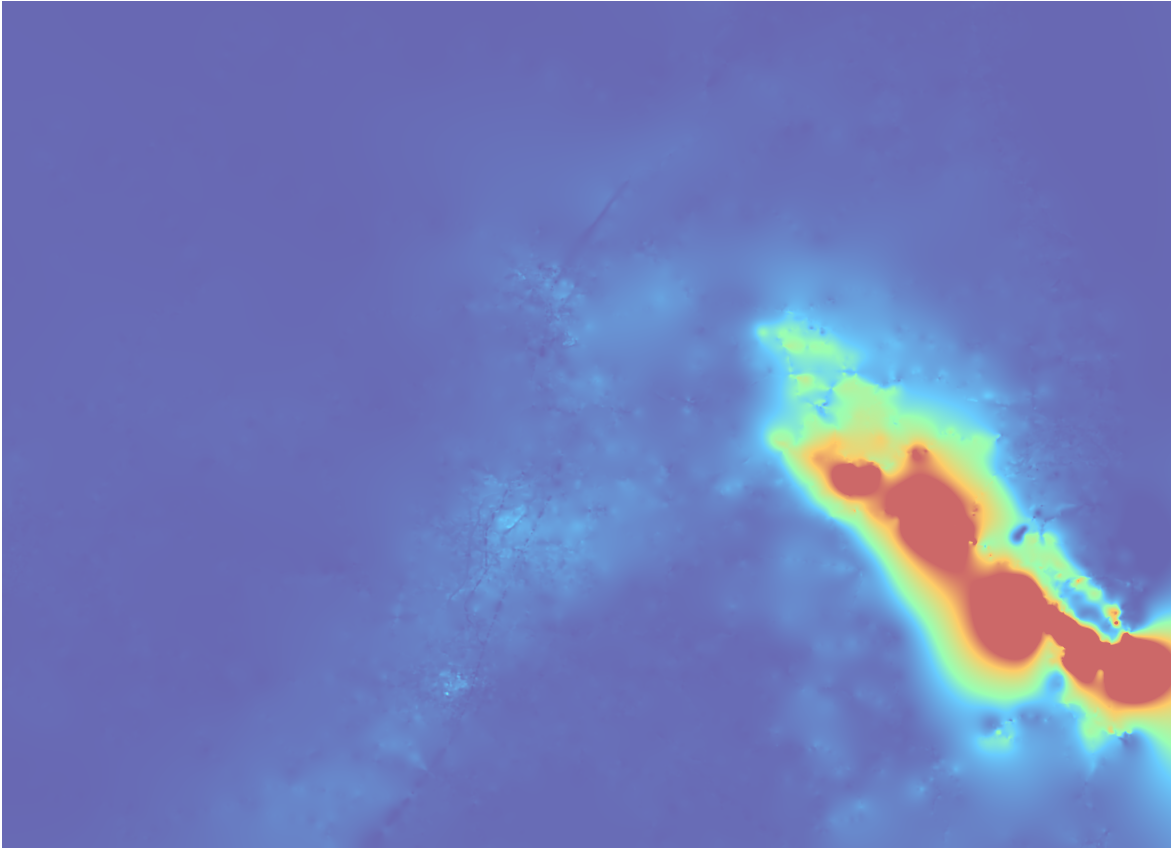
\includegraphics[scale=0.4]{./pictures/interpolovana_mapa.png}
      	\caption[Interpolovaná mapa dávkových příkonů (prefektura
Fukushima)]{Interpolovaná mapa dávkových příkonů gama záření
(prefektura Fukushima)}(zdroj: vlastní, data poskytnutá od SÚRO,
v.v.i.)
    	\label{fig:interpolatedMap}
\end{figure}

\subsection{Trasa monitorování} Trasy monitorování použité pro
testování byly naplánovány pomocí běžně používaných webových služeb
Mapy.cz a Google (jak již bylo zmíněno v~kapitole
\ref{subsec:vstupniData}). Trasy byly vyexportovány ve formátech
\zk{KML} a \zk{GPX}. Byly voleny tak, aby se jejich průběh co nejvíce
přiblížil \zk{JE} Fukushima a aby byla vidět výrazná změna hodnot
dávkových příkonů. Ukázku trasy monitorování lze nalézt v obr. \ref{fig:trasa}.
\newpage
\begin{figure}[H] \centering
    
\includegraphics[scale=0.3]{./pictures/trasa_monitorovani.png}
      	\caption[Trasa monitorování (Futaba-Nawashirogae, prefektura
Fukushima)]{Trasa monitorování (Futaba-Nawashirogae, prefektura
Fukushima)}(zdroj: vlastní, data poskytnutá od SÚRO, v.v.i.)
    	\label{fig:trasa}
\end{figure}

%%% ML: Chybi mi tu ukazky vystupu a zminka, ze vlastni navod na
%%% pouzit modulu je v priloze

%%% MK: Ukázky výstupu mám v podkapitole Výstupní data 

\section{Návod na použití}
K zásuvnému modulu byl vytvořen návod na použití v anglickém jazyce. 
Návod je uveden v příloze \textbf{B}. 
\chapter{Závěr}
\label{5-zaver}

Hlavním cílem této bakalářské práce byla implementace zásuvného modulu
do QGIS rozšiřujícího softwarové vybavení Státního ústavu pro radiační
ochranu v.v.i. (i~jiných institucí). Nástroj poslouží jako další
prostředek k~zrychlení reakční doby při cvičeních radiačních havárií
příp. při samotných radiačních haváriích a především k~zvýšení
bezpečnosti mobilních skupin pracujících přímo v~terénu. Dále si práce
kladla za cíl seznámit čtenáře s~dopady ionizujícího záření na lidský
organismus a s~metodou pozemního snímání radiace.

Vytvářený nástroj ze vstupní interpolované mapy dávkových příkonů gama
záření vyextrahuje data na dané trase a spočte několik základních
statistik. Zejména se jedná o~celkovou dávku gama záření, kterou
mobilní skupina na trase obdrží. V~případě překročení mezních hodnot
obdržené dávky, které již ohrožují na zdraví, je možné pomocí dalších
výsledků výpočtu vytipovat místa na trase, kterým se vyhnout a tedy
trasu monitorování modifikovat.

Nástroj byl s~pomocí návrhů a požadavků na úpravy od pracovníků
\zk{SÚRO} vytvořen na míru tak, aby splnil očekávání a byl zároveň co
nejvíce intuitivní. Nástroj byl vytvořen v~anglickém jazyce s~vidinou
jeho využití i v~jiných než českých institucích. Zároveň byl
v~angličtině vytvořen návod na jeho používání.


\section{Licence a dostupnost zásuvného modulu} Zásuvný modul byl
vytvořen pod licencí \zk{GNU GPL}, kterou podědil po QGIS knihovnách,
jež byly k~implementaci využity. Zásuvný modul je volně dostupný z~CTU
GeoForAll Lab QGIS
%%% ML: tady mate odkaz na online manual
%%% ML: mluvite o Git anebo QGIS repozitari (zde by mel byt odkaz na git)
repozitáře\footnote{\texttt{https://ctu-geoforall-lab-projects.github.io/bp-kala-2017/}}. V~budoucnu
je dále v~plánu začlenění zásuvného modulu do oficiálního QGIS
repozitáře.

 





% Vysázení seznamu zkratek

\begin{seznamzkratek}{ABCDE}

	\novazkratka{GNU GPL}
	      {GNU GPL}
	      {????}

	\novazkratka{SÚRO}
	      {SÚRO}
	      {Státní ústav radiační ochrany, v. v. i.}

	\novazkratka{SÚJB}
	      {SÚJB}
	      {Státní úřad pro jadernou bezpečnost}

	\novazkratka{CSV}
		  {CSV}
		  {Comma-separated values - hodnoty oddělené čárkou}
		  
	\novazkratka{KML}
		  {KML}
		  {Keyhole Markup Language}
		  
	\novazkratka{GPX}
		  {GPX}
		  {GPS Exchange Format}
	
	\novazkratka{JE}
		  {JE}
		  {Jaderná elektrárna}
		  
	\novazkratka{GIS}
		  {GIS}
		  {Grafický informační systém}
\end{seznamzkratek}

% Literatura
\nocite{*}
\def\refname{Literatura}
\bibliographystyle{mystyle}
\bibliography{literatura}


% Začátek příloh
\def\figurename{Figure}
\prilohy

% Vysázení seznamu příloh
%\seznampriloh

% Vložení souboru s přílohami
%%%%%%%%%%%%%%%%%%%%%%%%%%%%%%%%%%%%%%%%%%%%%%%%%%%%%%%%%%%%%%%%%%%%%%%%%%%%%%%%%%%
%%                 PŘÍLOHA - UŽIVATELSKÁ PŘÍRUČKA                                %%
%%%%%%%%%%%%%%%%%%%%%%%%%%%%%%%%%%%%%%%%%%%%%%%%%%%%%%%%%%%%%%%%%%%%%%%%%%%%%%%%%%%
\chapter{User guide}
\label{user-guide}

This user guide is ...

\section{Loading of plugin}
\label{plugin-load}




% Konec dokumentu
\end{document}
